\section{Validation of the Method with Mock Data}
\label{ap:mock-data}

Here we show the results of applying our density fitting technique to mock data, as described in \S~\ref{subsec:method-validation}. Figure~\ref{fig:mock_posterior} shows the posterior distributions for fits to mock data with and without disk contamination, as well as mock data created using kinematic cuts that mirror those used to select the \gse samples. The contours of the posterior distributions are set at 1 and 2-$\sigma$. The black lines show the input parameters for the models. The posterior distributions always contain the input model parameters, yet are broad in general. This is due to the fact that we chose to fit a lightweight mock halo (only $2\times10^{8}$~M$_{\odot}$ total mass) to test whether our modelling approach would work with a small number of stars. Since each stellar halo realization is subject to a certain degree of randomness we generate multiple stellar halos with similar parameters and a variety of masses. We find that the input parameters are always contained in the posterior, and that there are no major systematic over- or underestimations of input parameters beyond those noted in \S~\ref{subsec:method-validation}.

\begin{figure*}
    \centering
    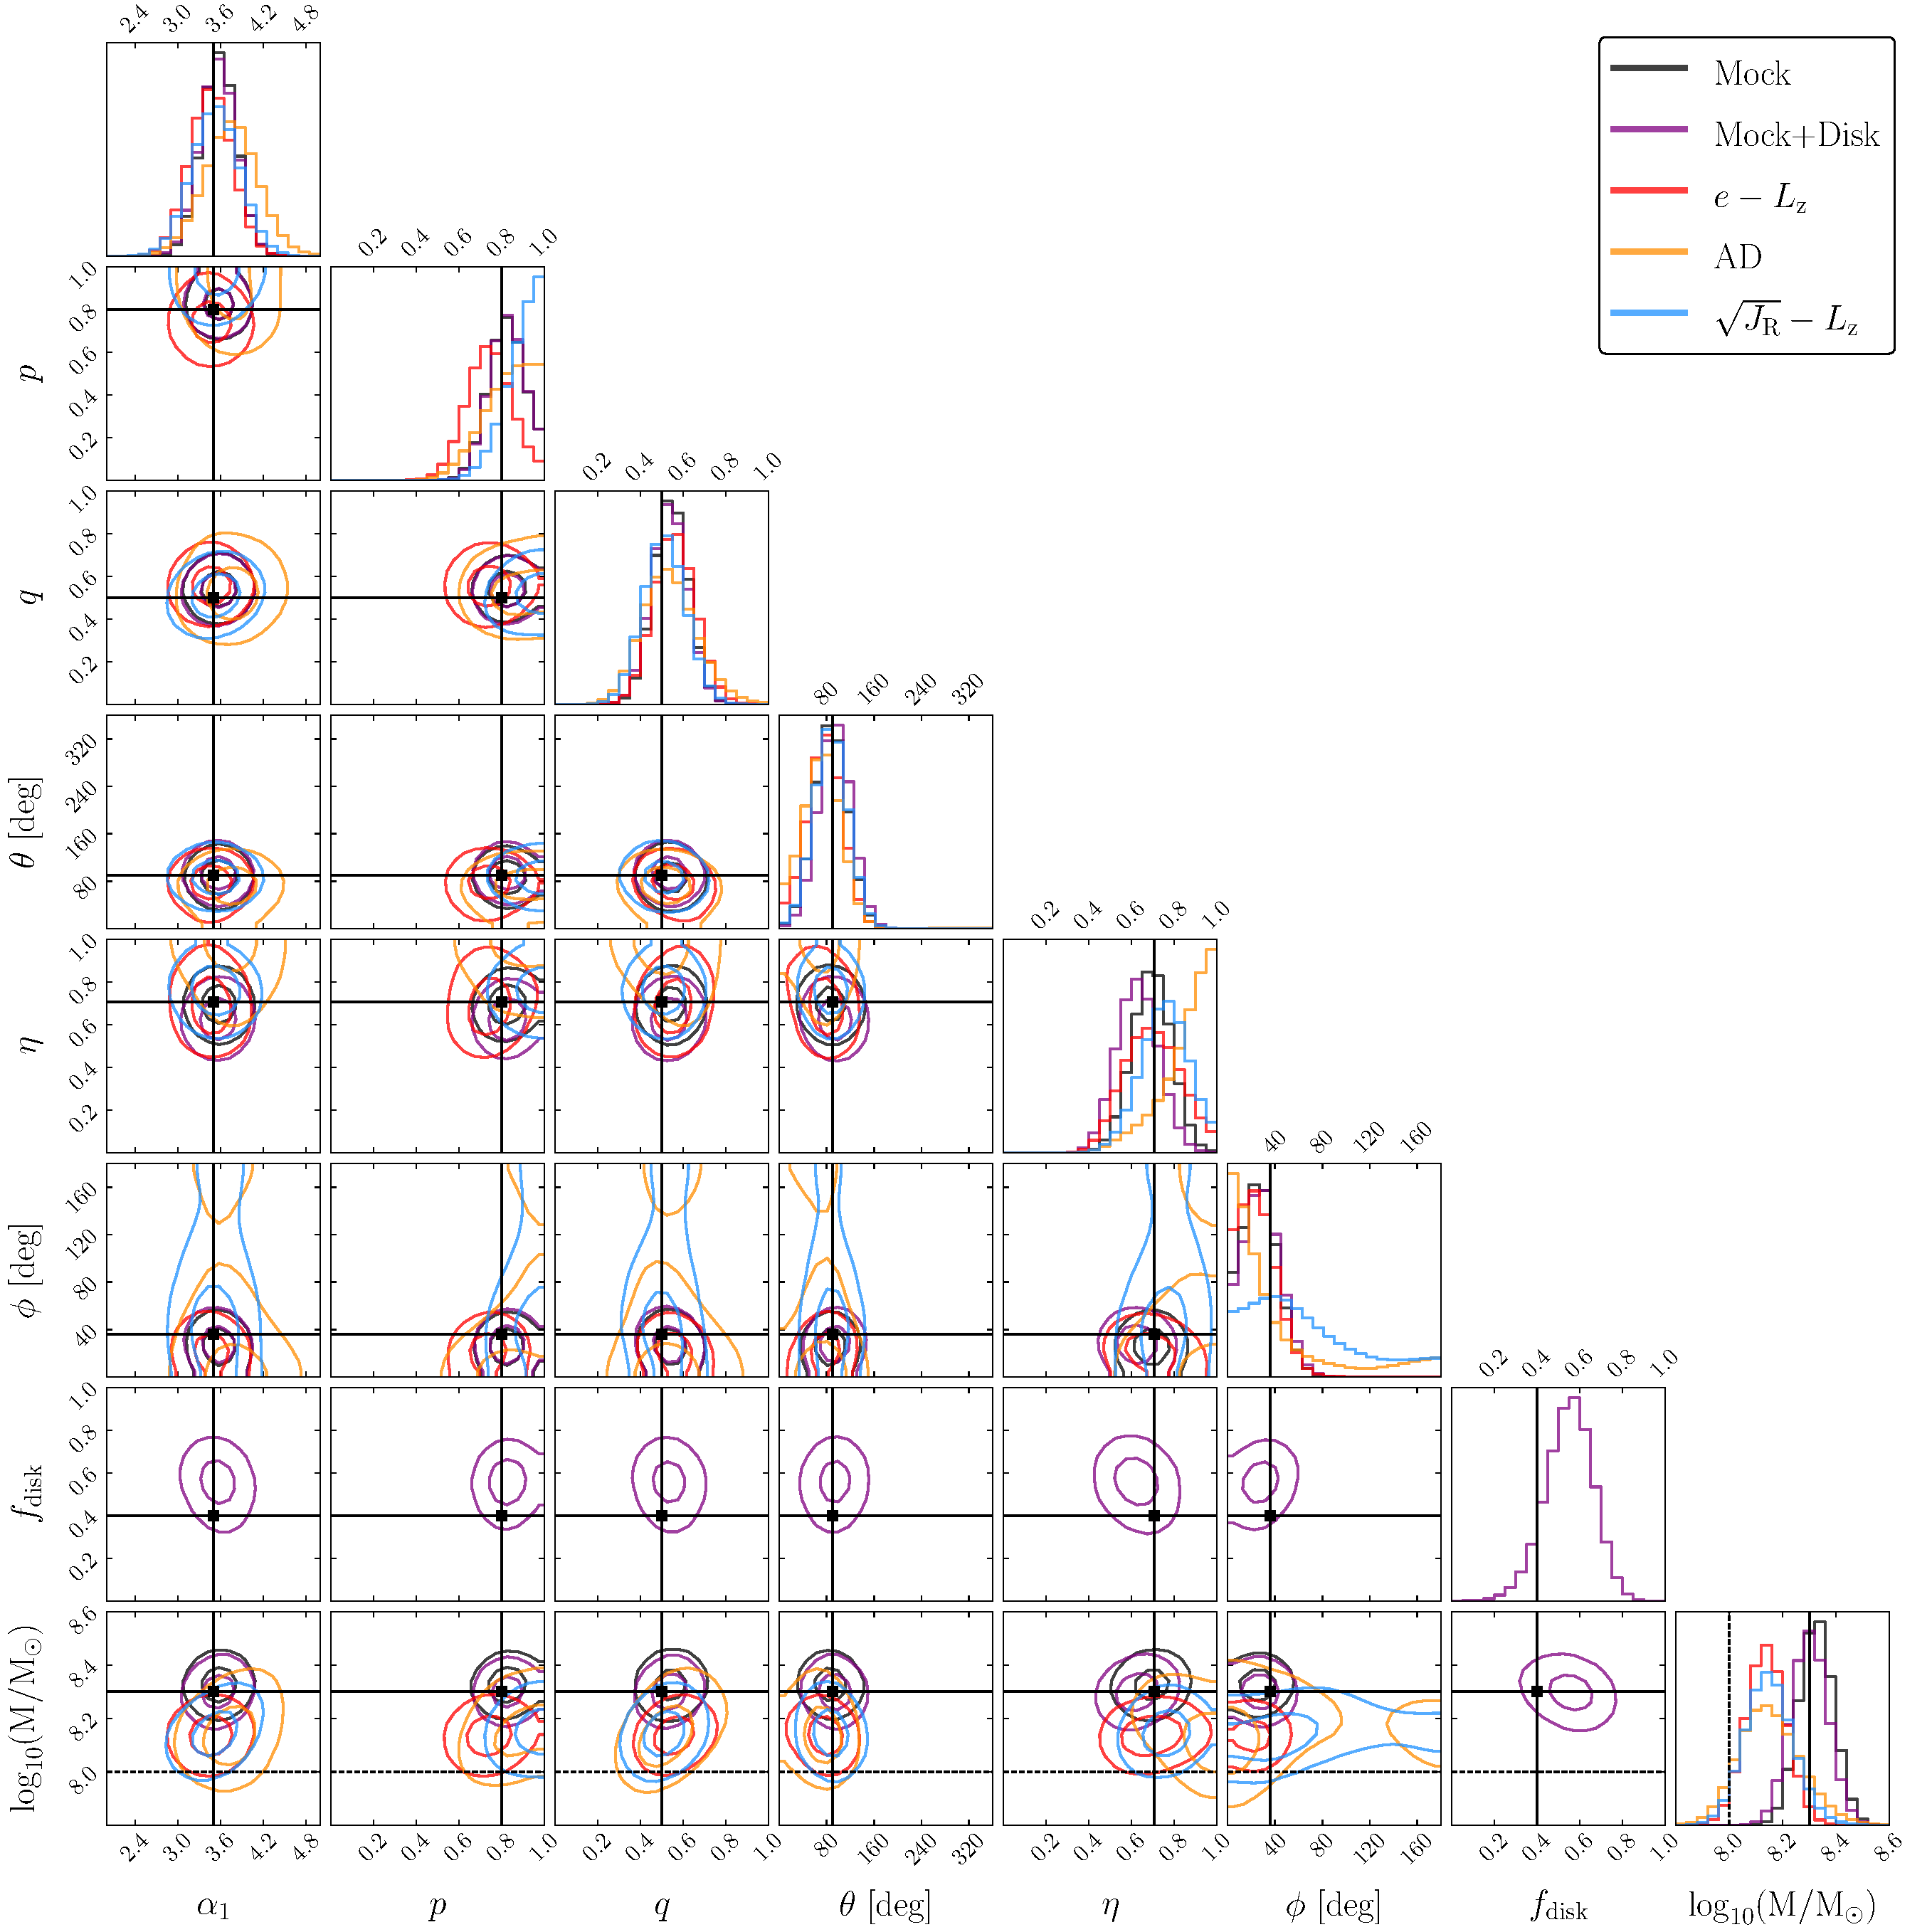
\includegraphics[width=\halftextwidth]{figure/ch3/mock_posterior.pdf}
    \caption{Corner plot showing the posterior samples of the fits to mock data. Contours are placed at the 1 and 2-$\sigma$ levels. The black lines show the fit to the whole mock sample without disk contamination, the grey line shows the fit including to the whole sample including disk contamination, and the coloured lines show the fits to the mock \gse kinematic samples without disk contamination. the solid black lines show the input parameters for the models, and the dashed black lines show the mass expected for the kinematically selected \gse analog populations (half that of the whole mock).}
    \label{fig:mock_posterior}
\end{figure*}

\section{Completeness of the modified kinematic effective selection function}
\label{ap:modified-ksf}

Here we show the kinematic effective selection function derived based on our fits to the \gse and whole-halo populations described in \S~\ref{subsec:altering-kinematic-effective-selection-function}. Figures~\ref{fig:ksf2_dmod_fields} and \ref{fig:ksf2_lb_dmod_marginalized} are identical to Figures~\ref{fig:ksf_dmod_fields} and \ref{fig:ksf_lb_dmod_marginalized}, except they use this new kinematic effective selection function (denoted $\mathfrak{S}_{2}^{\prime}$). On to Figure~\ref{fig:ksf2_dmod_fields} we add the median of $\mathfrak{S}_{2}^{\prime}$ and $\mathfrak{S}_{2}$, calculated across all fields at each distance modulus, to aid efficient comparison of typical values.

\begin{figure*}
    \centering
    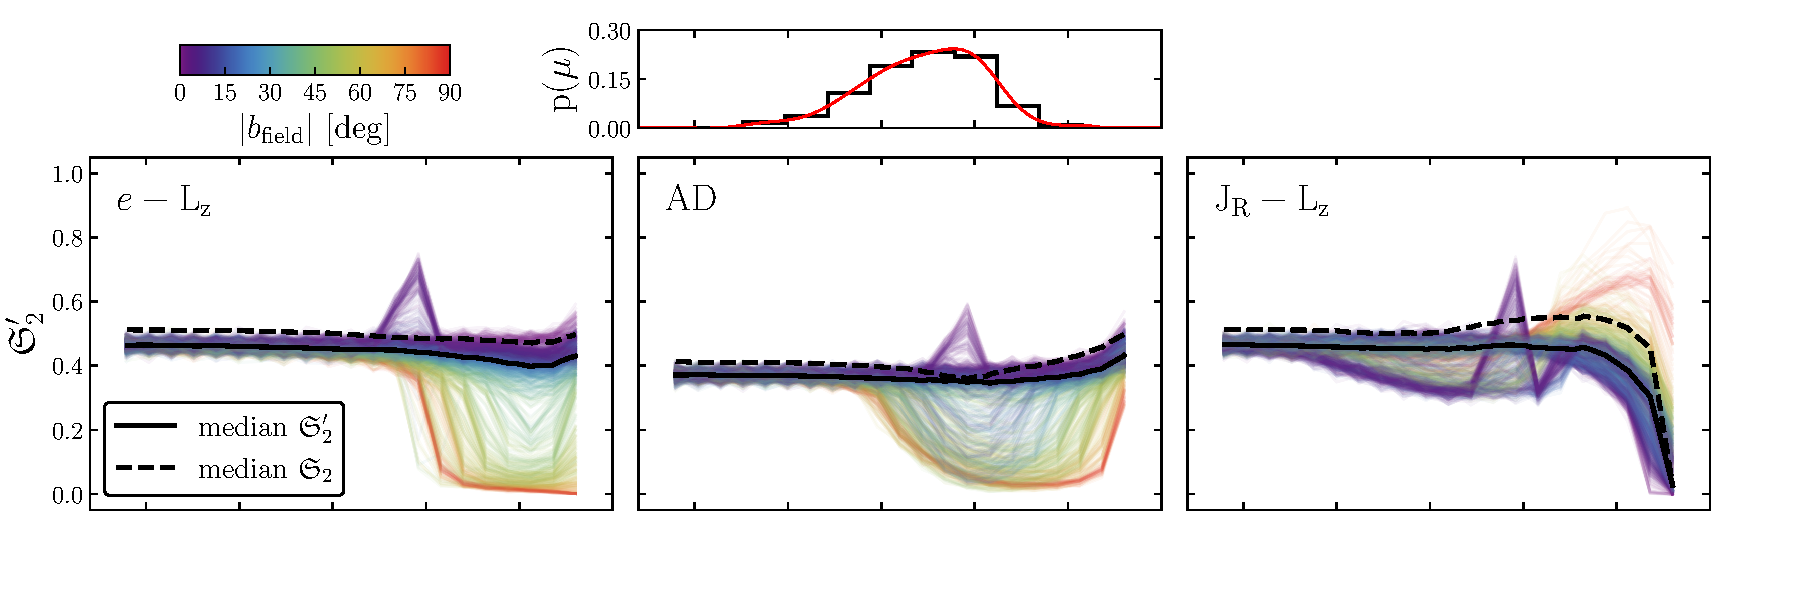
\includegraphics[width=\halftextwidth]{figure/ch3/ksf2_dmod_fields.pdf}
    \caption{Same as Figure~\ref{fig:ksf_dmod_fields} but for the secondary kinematic effective selection function (denoted $\mathfrak{S}_{2}^{\prime}$) described in \S~\ref{subsec:altering-kinematic-effective-selection-function}. Overlaid on each panel are the median, calculated at each distane modulus, both of this secondary kinematic effective selection function $\mathfrak{S}_{2}^{\prime}$ (black solid line) and the original kinematic effective selection function $\mathfrak{S}_{2}$ (black dashed line) presented in Figure~\ref{fig:ksf2_dmod_fields}.}
    \label{fig:ksf2_dmod_fields}
\end{figure*}

\begin{figure}
    \centering
    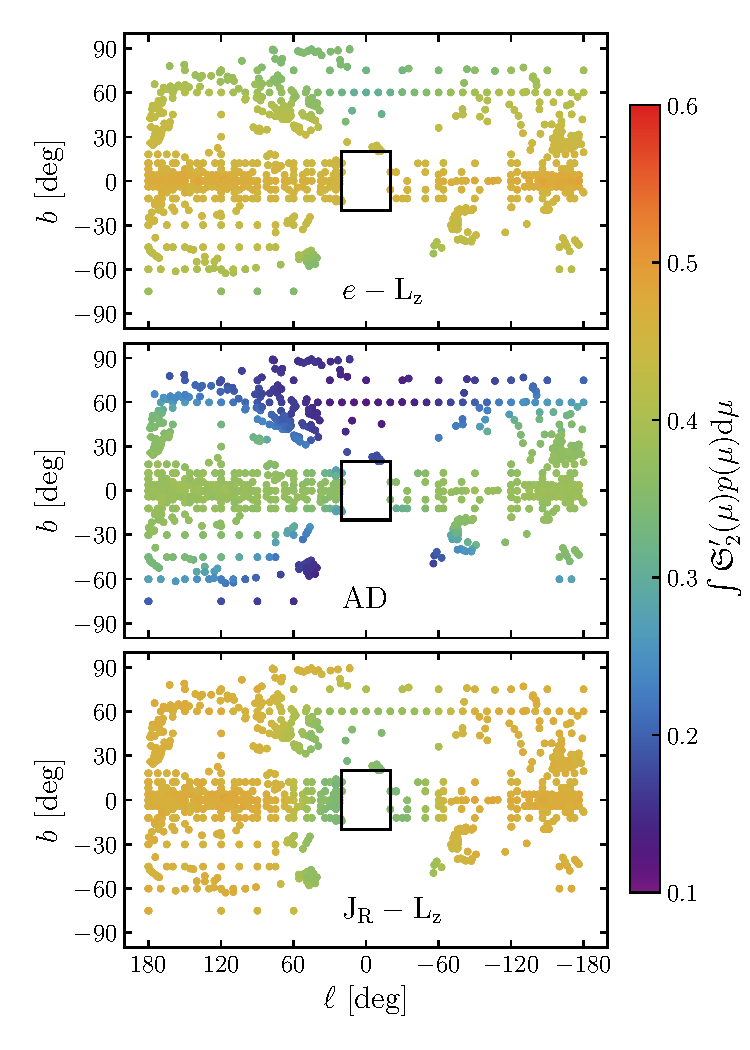
\includegraphics[width=\halftextwidth]{figure/ch3/ksf2_lb_dmod_marginalized.pdf}
    \caption{Same as Figure~\ref{fig:ksf_lb_dmod_marginalized} but for the secondary kinematic effective selection function described in \S~\ref{subsec:altering-kinematic-effective-selection-function}.}
    \label{fig:ksf2_lb_dmod_marginalized}
\end{figure}